\documentclass{article}

\newcommand{\labduedate}{at the end of Week 4}

% Actual required things start here
\usepackage{array}
\usepackage{mdwlist}
\usepackage{fancyhdr}
\usepackage[usenames,dvipsnames]{color}
\usepackage{graphicx}
\usepackage{minted}
\usepackage{fullpage}
\usepackage[colorlinks=true]{hyperref}
\usepackage{textcomp}
\usepackage{totcount}

% Helpful shortcuts for the document itself
\newcommand{\productname}{MoteView}
\newcommand{\longproductname}{Crossbow MoteView 2.0F r21}
\newcommand{\labnumber}{2}


\newtotcounter{questions}\setcounter{questions}{0}
\newcommand{\question}[1]{
\addtocounter{questions}{1}
\ifnum1=#1
\textbf{[Question \arabic{questions} \textrm{\textit{(#1 pt)}}] }
\else
\textbf{[Question \arabic{questions} \textrm{\textit{(#1 pts)}}] }
\fi
}

\newtotcounter{tasks}\setcounter{tasks}{0}
\newcommand{\task}[2]{
\addtocounter{tasks}{1}
\setcounter{subtasks}{0}
\ifnum0=#1
\subsection*{Task \arabic{tasks}: #2}
\else
\subsection*{Task \arabic{tasks}: #2 \textit{(#1 pts)}}
\fi
}

\newtotcounter{subtasks}\setcounter{subtasks}{0}
\newcommand{\subtask}[2]{
\addtocounter{subtasks}{1}
\ifnum0=#1
\subsubsection*{Subtask \arabic{tasks}.\arabic{subtasks}: #2}
\else
\subsubsection*{Task \arabic{tasks}.\arabic{subtasks}: #2 \textit{(#1 pts)}}
\fi
}

\pagestyle{fancy}
\headheight 24pt
\begin{document}

\chead{\textcolor{Gray}{CSSE491 -- Mesh Networking Lab Assignment}}
\headsep = 24pt

\begin{center}
{ \large
\textbf{Lab \labnumber: \longproductname} \\
\textbf{MoteMap}
}
\end{center}

\subsection*{Objective}
This lab deals with the visualization of mote data for end users, and as such it takes a turn from previous work with MoteView into a web-based application. By the end of this lab, you should be able to demonstrate how changes in mote data are reflected in a web-based visualizer, and propose ideas for how visualization of mote data can be applied to real-world situations.

\subsection*{Lab format}
This lab is primarily guided; it serves mostly as instructional material for students learning to interpret mote data. Like the previous lab, however, it is interspersed with comprehension questions and has some minor individual components.

Note that this lab provides a significant amount of flexibility, compared to earlier labs. \textbf{You will be expected to adapt these lab instructions to your own setup and troubleshoot problems on your own.} We cannot possibly cover every different configuration that your mesh setup can be in; as such, we provide a general outline in this lab, and ask that you \textbf{think carefully through these instructions} and \textbf{apply them as appropriate}.

\subsection*{Required materials}
For this lab, you will need:

\begin{itemize*}
\item The configured Windows XP SP3 system from Lab 0
\item A MIB520 control board with an IRIS mote
\item At least three other IRIS motes, each with its own MDA100CB sensor board
\end{itemize*}

You will also benefit greatly from having a working installation of Ruby 1.9; this lab will provide brief instructions for installing Ruby, but having a copy already set up will speed up the lab immensely.

\subsection*{Grading rubric}
\begin{tabular}{p{5.5in} r}
Tasks 1 and 3 are worth \textbf{10} points each. & $2 \times 10 = 20$ \\
Task 2 is worth \textbf{5} points. & $1 \times 5 = 5$ \\
Questions 1-4 are worth \textbf{5} points each. & $4 \times 5 = 20$ \\
Question 5 is worth \textbf{10} points. & $1 \times 10 = 10$ \\
You may earn \textbf{20} points extra credit. & $1 \times 20 = 20$ \\ \hline
& \textbf{55} points (up to \textbf{75})
\end{tabular}

\subsection*{Due date}
The lab is due \textcolor{red}{\textbf{\labduedate}}.

\subsection*{Turn-in instructions}
Create a new folder and add the following files to it:
\begin{itemize}
\item Edited project files from \productname, if any
\item A PDF file with the answers to each question \textit{clearly marked}. When you have completed this lab, you will have answered \total{questions} questions.
\item A \verb!who.txt! file with your name. If you worked with someone else, include their name in the \verb!who.txt! file.
\end{itemize}

Once your work is done and in the folder, zip the entire folder and submit it on ANGEL. You may work with a partner, as long as each of you submits your own copy of all of the listed files. Note that files submitted via email or other methods will receive zero credit. In addition, files that cannot be accessed without additional work (e.g. non-zip archives or LaTeX documents that require compiling) will lose you points. After you submit your files, please complete the feedback survey on Angel Under Labs - Labs Anonymous Feedback!


\subsection*{Architecture}

Before we begin, let's take a second and consider the architecture of the system this lab will build. We've already been capturing data from a mesh network using MoteView; behind the scenes, MoteView uses \href{http://www.postgresql.org/}{PostgreSQL}, a freely available open-source database engine, to store data from motes. In this lab, we'll be connecting to that PostgreSQL database using a Ruby web application, then accessing that application in a web browser to view mote data in a visual format. This architecture is captured below:

\begin{center}
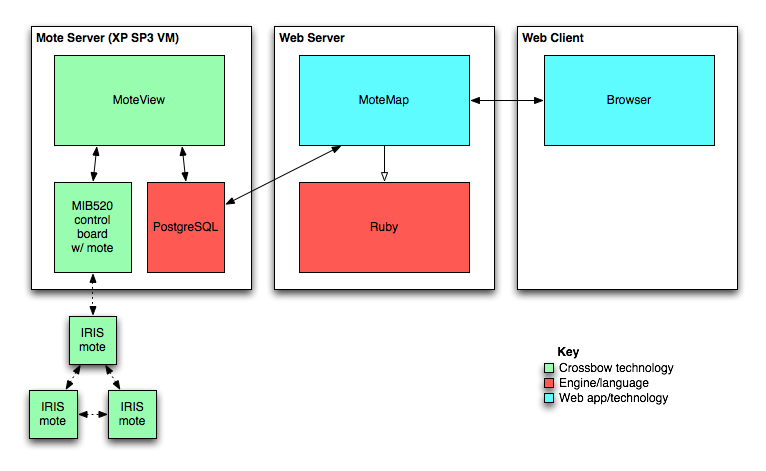
\includegraphics[width=6in]{arch.png}
\end{center}

The sections in green have been covered in past labs; those in red are new in this lab, but are so-called ``backbone'' technologies and are not particularly relevant in and of themselves; and the sections in blue are where we focus most of our work in this lab.

\task{10}{Install Software}

Though PostgreSQL is already installed (with the Crossbow suite of applications), we must install Ruby before the MoteMap web application will run. The installation process is somewhat out of scope for this lab; in most cases, however, the following should suffice:

\begin{itemize}
\item Windows users can get the Ruby installer from \href{http://rubyinstaller.org/}{rubyinstaller.org}; it should be entirely self-contained for most Windows setups. After installation, verify that you can access the \verb!ruby! and \verb!gem! commands from a standard command prompt.
\item Mac users have Ruby 1.8 installed by default; for this lab, you must install \href{http://mxcl.github.com/homebrew/}{Homebrew}, then \verb!brew install ruby!. Ensure that the \verb!ruby! executable accessed from a shell is version 1.9; you may have to alter your \verb!PATH!.
\end{itemize}

After installing Ruby 1.9, use the \verb!gem! command to install the necessary gems. (On Windows, you may also need the \href{http://rubyinstaller.org/add-ons/devkit/}{Ruby DevKit} before the installation will work.) Run the following commands:

\begin{verbatim}
gem install sinatra
gem install haml
gem install sass
gem install pg
gem install json
gem install data_mapper
gem install parseconfig
\end{verbatim}

Finally, you will also need the Git source control management tool. There are installers available for both \href{http://msysgit.github.com/}{Windows} and \href{http://code.google.com/p/git-osx-installer/}{Mac}; alternately, Mac users can use Homebrew to \verb!brew install git!.

If you have any trouble installing Ruby, DevKit (Windows only), any of the gems, or Git, inform a TA or your instructor.

\task{5}{Configure Network}

Now that you have all the necessary software to run the MoteMap application, you will need to configure the network so that PostgreSQL is accessible. Let's name our computers for easier reference:

\begin{itemize*}
\item The \textbf{mote server} is the Windows XP machine running MoteView and hosting the PostgreSQL database; for most of you, this is a virtual machine.
\item The \textbf{web server} is the machine with Ruby and its gems installed; generally, this is the machine hosting the mote server VM (i.e. running VirtualBox).
\item The \textbf{web client} is the machine you will be accessing MoteMap from. This can be any machine with a web browser; for simplicity, it is usually the same as the web server.
\end{itemize*}

With that naming out of the way, the goal of this task is simple: allow the web server access to port 5432 on the mote server. The process of doing so will vary, depending on how you have your machines configured. Find the item below that applies to you, and follow its instructions.

\begin{itemize}
\item If both your mote server and web server are the same machine (i.e., you are installing Ruby and MoteMap on your XP machine), merely open port 5432 in your Windows Firewall configuration.
\item If your web server is the same as the machine hosting your mote server's VM, you will need to open port 5432 in your Windows Firewall configuration on the mote server, then forward localhost (127.0.0.1) port 5432 from your host machine to the mote server's port 5432. In VirtualBox, this is done through your machine's networking settings.
\item If your mote server and web server are separate physical machines, open port 5432 in your Windows Firewall configuration, then ensure you can establish a network connection between the two servers; they must be able to create an IP connection before you continue.
\end{itemize}

\task{10}{Install MoteMap}

Now that your networking is configured, a copy of the MoteMap application should be able to access the PostgreSQL database managed by MoteView on your mote server. We can now go ahead and install MoteMap; create a new folder for the application, then (in a shell) move to that folder and execute:

\begin{verbatim}
git clone https://github.com/lithium3141/MoteMap.git
\end{verbatim}

This will copy the MoteMap application from its upstream location to a new folder on your machine. Move into that folder and examine the file \verb!postgres.conf!; you will need to populate this file with the proper host for your PostgreSQL database. The default value, \verb!localhost!, will suffice for all cases except if your mote server and web server are two separate physical machines; in that case, change \verb!localhost! to the hostname or IP address of your mote server. (Windows users may need an advanced text editor, such as \href{http://notepad-plus-plus.org/}{Notepad++}, to view this file properly.)

Once your configuration is set up, launch the MoteMap application by running:

\begin{verbatim}
ruby motemap.rb
\end{verbatim}

You should see output similar to the following:

\begin{verbatim}
== Sinatra/1.3.2 has taken the stage on 4567 for development with backup from Thin
>> Thin web server (v1.3.1 codename Triple Espresso)
>> Maximum connections set to 1024
>> Listening on 0.0.0.0:4567, CTRL+C to stop
\end{verbatim}

This indicates that the webapp has launched successfully. If you have trouble, or see any errors in your console, attempt to resolve them yourself; if you are unsure what an error means, or cannot find a solution via Google, contact an instructor or TA. Once everything is taken care of, go to the home page of the MoteMap application in a web browser; for most people, this will be \href{http://localhost:4567}{localhost:4567}. After a few seconds, you should see MoteMap create motes on the screen and begin populating them with data.

MoteMap will update mote data live from incoming results; following instructions from Lab 2, establish a small mesh network using the MDA100CB sensor boards, and ensure that MoteView is running and capturing data. Once you see MoteMap nodes on-screen and MoteView is capturing information from the motes, please answer the following questions:

\question{5} Experiment with your motes -- can you tell what the two sides of a mote represent in MoteMap? Can you influence the data shown in MoteMap?

\question{5} Turn one mote off for a period of time. Does anything change about its MoteMap representation? What do you think this represents?

\question{5} Append \verb!/background/set! to the MoteMap URL. Upload a background image of your choosing. How might you use a background to provide more contextual information for your mesh network?

\question{5} Look through the source code for the MoteMap application; focus specifically on the \verb!routes/api/node.rb! file. What additional information can you find in MoteMap? What URLs should you access to get that data?

\question{10} Write a short paragraph explaining an idea for applying your mesh network and MoteMap to a real-world situation or problem. How might live data updates, visualized for end users, be beneficial?

\subsection*{Extra Credit}

If you are interested in earning extra points on this lab, you can read the MoteMap source code and contribute something to the application. Consider fixing a bug that is \href{https://github.com/lithium3141/MoteMap/issues}{outstanding on the application} or adding a new feature of your own. For full credit, fork the MoteMap repository to your own GitHub account, then submit a pull request to have your work merged back into the master application. You may earn up to 20 points extra credit by completing this section.

\subsection*{Turn-in instructions}
Create a new folder and add the following files to it:
\begin{itemize}
\item Edited project files from \productname, if any
\item A PDF file with the answers to each question \textit{clearly marked}. When you have completed this lab, you will have answered \total{questions} questions.
\item A \verb!who.txt! file with your name. If you worked with someone else, include their name in the \verb!who.txt! file.
\end{itemize}

Once your work is done and in the folder, zip the entire folder and submit it on ANGEL. You may work with a partner, as long as each of you submits your own copy of all of the listed files. Note that files submitted via email or other methods will receive zero credit. In addition, files that cannot be accessed without additional work (e.g. non-zip archives or LaTeX documents that require compiling) will lose you points. After you submit your files, please complete the feedback survey on Angel Under Labs - Labs Anonymous Feedback!


\subsection*{Revision History}
\begin{itemize*}
\item Mon May 14 12:15:27 EDT 2012: Lab written by Tim Ekl
\end{itemize*}

\end{document}
